\documentclass{beamer}
\usepackage[utf8]{inputenc}
\usepackage{graphicx}

\hypersetup{
    colorlinks,%
    citecolor=blue,%
    filecolor=blue,%
    linkcolor=blue,%
    urlcolor=blue 
    %urlcolor=mygreylink     % can put red here to better visualize the links
}

\author[Sowmya Vajjala]{Instructor: Sowmya Vajjala}

\title[LING 520]{LING 520: Computational Analysis of English}
\subtitle{Semester: FALL '16}

\date{4 October 2016}

\institute{Iowa State University, USA}
%%%%%%%%%%%%%%%%%%%%%%%%%%%

\begin{document}

\begin{frame}\titlepage
\end{frame}

\begin{frame}
\frametitle{Class Outline}
\begin{itemize}
\item Quick recap and conclusion of HMM Tagging
\item Assignment 3: Discussion about Problem 1
\item Transformation Based Learning
\item Evaluating POS taggers
\item Practice with POS taggers in NLTK
\end{itemize}
\end{frame}

\begin{frame}
\frametitle{}
\begin{center}
\Large HMM tagging
\end{center}
\end{frame}

\begin{frame}
\frametitle{HMM Tagging}
\begin{itemize}
\item Aim: Maximize the probability of a tag sequence, given a word sequence.
\\ $\hat t_1^n$ = argmax$_{t_1^n}$(P(w$_1^n|$t$_1^n$)*P(t$_1^n$))
\item First assumption: probability of a word depends only on its POS tag, not on previous words or tags.
\\ $\Rightarrow$ \small{P(w$_1^n|$t$_1^n$)} \normalsize $\approx$ $\pi_{i=1}^n$ \small{P(w$_i|$t$_i$)} \normalsize
\item Second assumption: probability of a tag appearing is only dependent on previous tag instead of entire history (for Bigram taggers!)
\\ $\Rightarrow$ \small{P(t$_1^n$)} \normalsize $\approx$ $\pi_{i=1}^n$ \small{P(t$_i|$t$_{i-1}$)} \normalsize
\item Considering these assumptions, $\hat t_1^n$ becomes: argmax$_{t_1^n} \pi_{i=1}^n$(P(w$_i|$t$_i$)*P(t$_i|$t$_{i-1}$))
\end{itemize}
\end{frame}

\begin{frame}
\frametitle{What does this mean in normal language?}
\begin{itemize}
\item This is the equation we have: \\ $\hat t_1^n$ = argmax$_{t_1^n} \pi_{i=1}^n$(P(w$_i|$t$_i$)*P(t$_i|$t$_{i-1}$))
\item (P(w$_i|$t$_i$) = Count(t$_i,w_i$)/Count(t$_i$)
\\ $\Rightarrow$ P(good$|$ADJ) = C(ADJ,good)/C(ADJ)
\item P(t$_i|$t$_{i-1}$) = Count(t$_{i-1},t_i$)/Count(t$_{i-1}$) (Same as in language models)
\\  $\Rightarrow$  P(NN$|$DT) = C(DT,NN)/C(DT)
\item This is HMM tagging. The "Hidden" here refers to the tag sequence, because that is something that we cannot observe in the input which is only a sequence of words.
\item If we use HMM for speech recognition, "observed" state is speech sequence, hidden state is word sequence.
\end{itemize}
\end{frame}

\begin{frame}
\frametitle{HMM - Example}
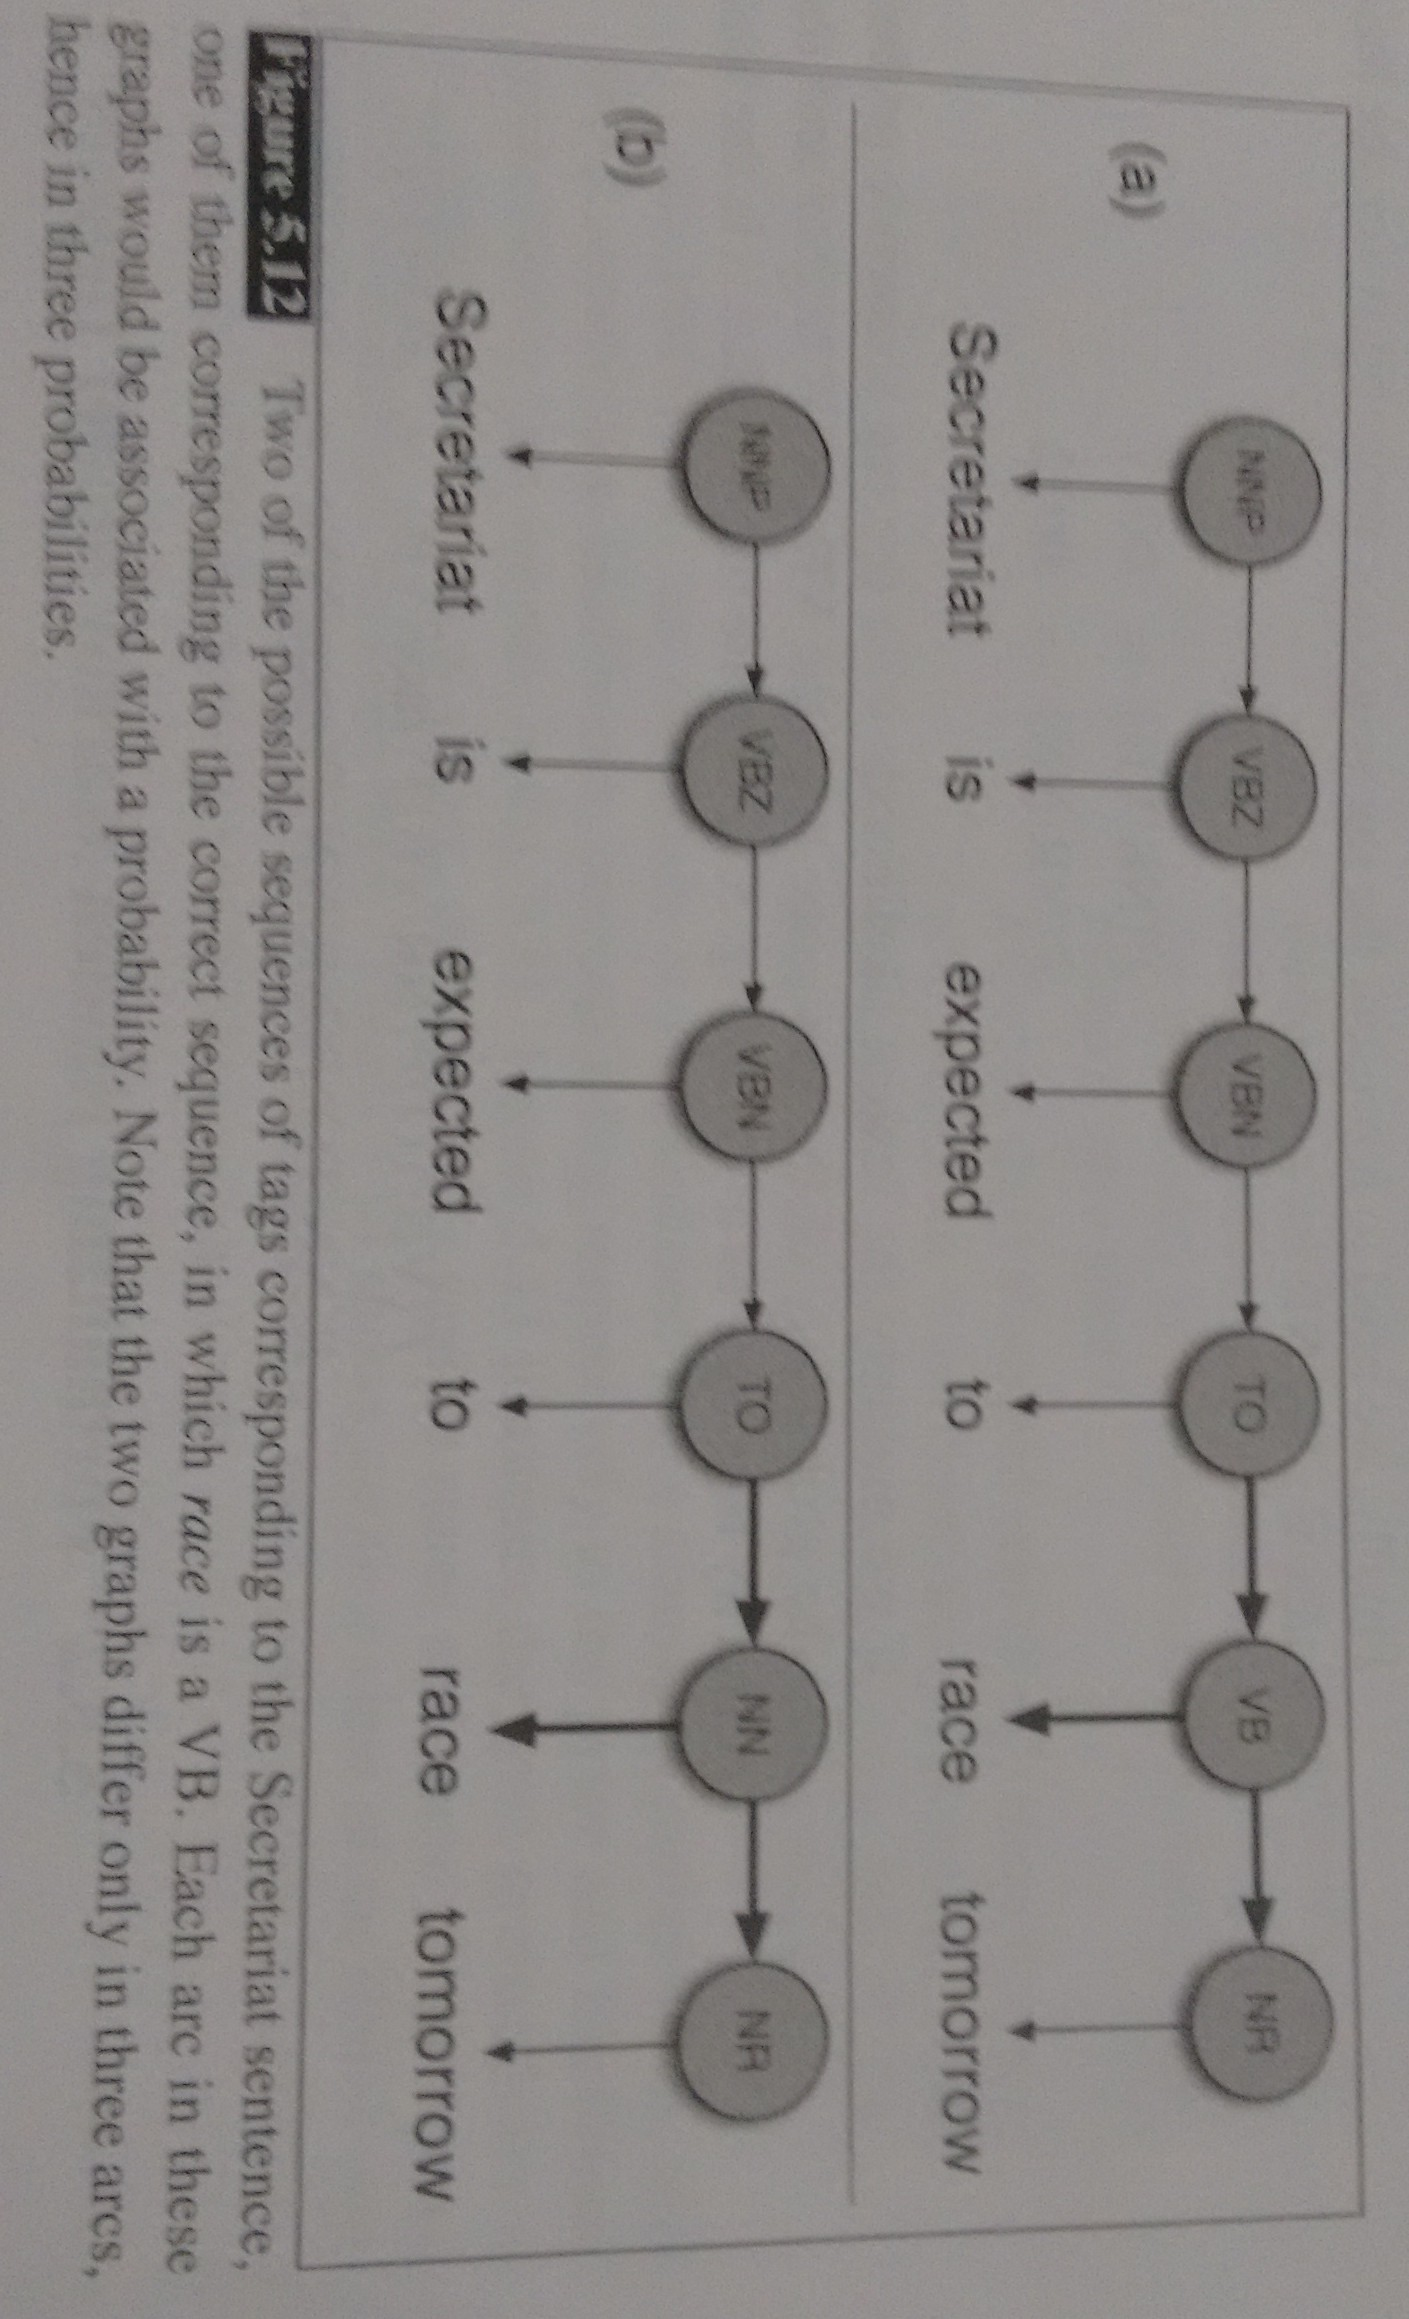
\includegraphics[width=0.4\textwidth,angle=90]{HMM-1.jpg}
\begin{itemize}
\item Only difference between the two tag sequence probabilities:
\begin{enumerate}
\item In sentence a), we estimate P(VB$|$TO)*P(NR$|$VB)*P(race$|$VB)
\item In sentence b), we estimate P(NN$|$TO)*P(NR$|$NN)*P(race$|$NN) instead.
\end{enumerate}
\end{itemize}
\end{frame}

\begin{frame}
\frametitle{HMM - What we need while training a model}
\begin{itemize}
\item Tag transition probabilities (e.g.,  P(NN$|$ADJ), P(VB$|$NN) etc. for a bigram model)
\item Observation likelihoods (e.g., P(race$|$VB), P(I$|$PRP) etc. for a bigram model)
\end{itemize}
- Once you build information about all these probabilities, you will just use these as a basis to tag a new sequence.
\end{frame}

\begin{frame}
\frametitle{Viterbi Algorithm for HMM }
\begin{itemize}
\item The task of determining which sequence of output is the most probable for input sequence is called decoding.
\item Viterbi algorithm is the most commonly used decoding algorithm for HMMs. 
\item This is also a form of dynamic programming (breaking up the problem into smaller problems and solving them one by one)
\item Viterbi algorithm provides an optimal solution of using all those tag-transition probabilities and observation likelihoods and finds the tag sequence which satisfies the maximum likelihood requirement to observation sequence. 
\end{itemize}
Note: Implementation details are beyond the scope of this course. Please read Chapter 5 and 6 in J\&M if you are interested to know more (and can handle more math)
\end{frame}

\begin{frame}
\frametitle{Assignment 3, Q1 - Overview and Hints}
\begin{itemize}
\item As mentioned on thursday, I want you to implement a trigram tagger of the kind: P(Tag2$|$Tag1,Word2). Not a HMM. If you want, you can implement a HMM instead.
\item What you need for this non-HMM trigram tagger: First, using the training data, you should create a file that can store this kind of counts: C(Tag1,Word2,Tag2)
\item The second program should be able to read these counts, and then, look at each word in the text sentence, grab the necessary counts, pick the trigram with maximum counts. 
\item Questions: How do we estimate probability for the first POS tag?? What do we do when we do not see a Trigram we want?? \pause
\item A small example of how it can look (without Erk's code, without NLTK.). 
\end{itemize}
\end{frame}

\begin{frame}
\frametitle{}
\begin{center}
\Large Transformation based tagging
\end{center}
\end{frame}

\begin{frame}
\frametitle{Tranformation Based Learning}
\begin{itemize}
\item TBL is a machine learning approach which relies both on the creation of rules, and inducing such rules automatically from a large annotated corpus.
\\ (Annotation here refers to POS tags.)
\item TBL occurs in three steps in the training phase:
\begin{enumerate}
\item Stage 1: Label every word with its most likely tag.
\item Stage 2: Automatically induce a set of rules based on pre-defined templates, to improve tagging from Step 1. (More on this in the next slide!)
\item Stage 3: Use these rules from Step 2 to re-tag sentences from Step 1. Repeat the rule induction and retagging process until there is no significant improvement in Tagger accuracy between two repeats.
\end{enumerate}
\end{itemize}
\end{frame}

\begin{frame}
\frametitle{Brill (1995)'s templates}
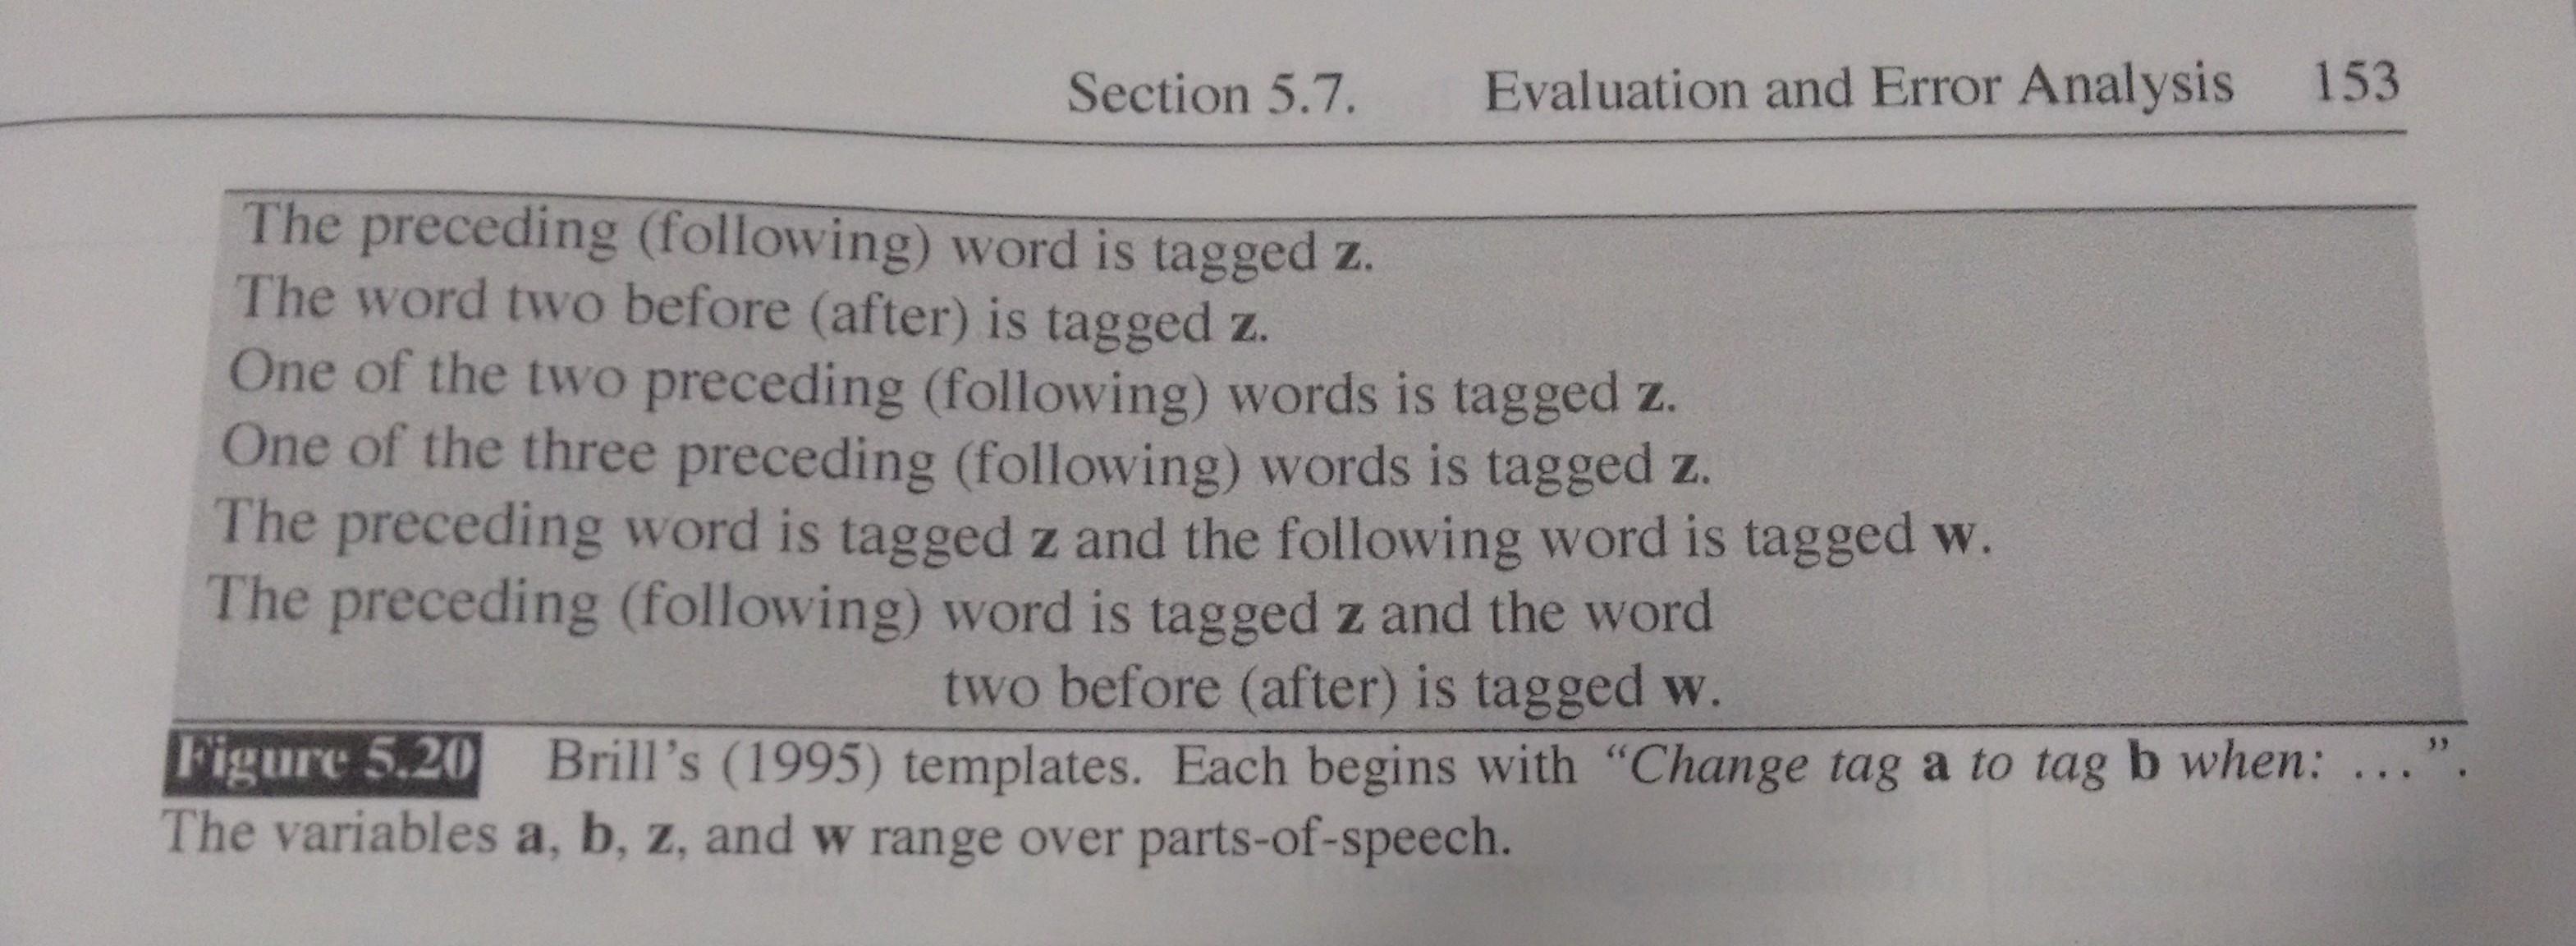
\includegraphics[width=0.9\textwidth]{Brill-1.jpg}
\end{frame}

\begin{frame}
\frametitle{Brill Tagger - Learned Rules}
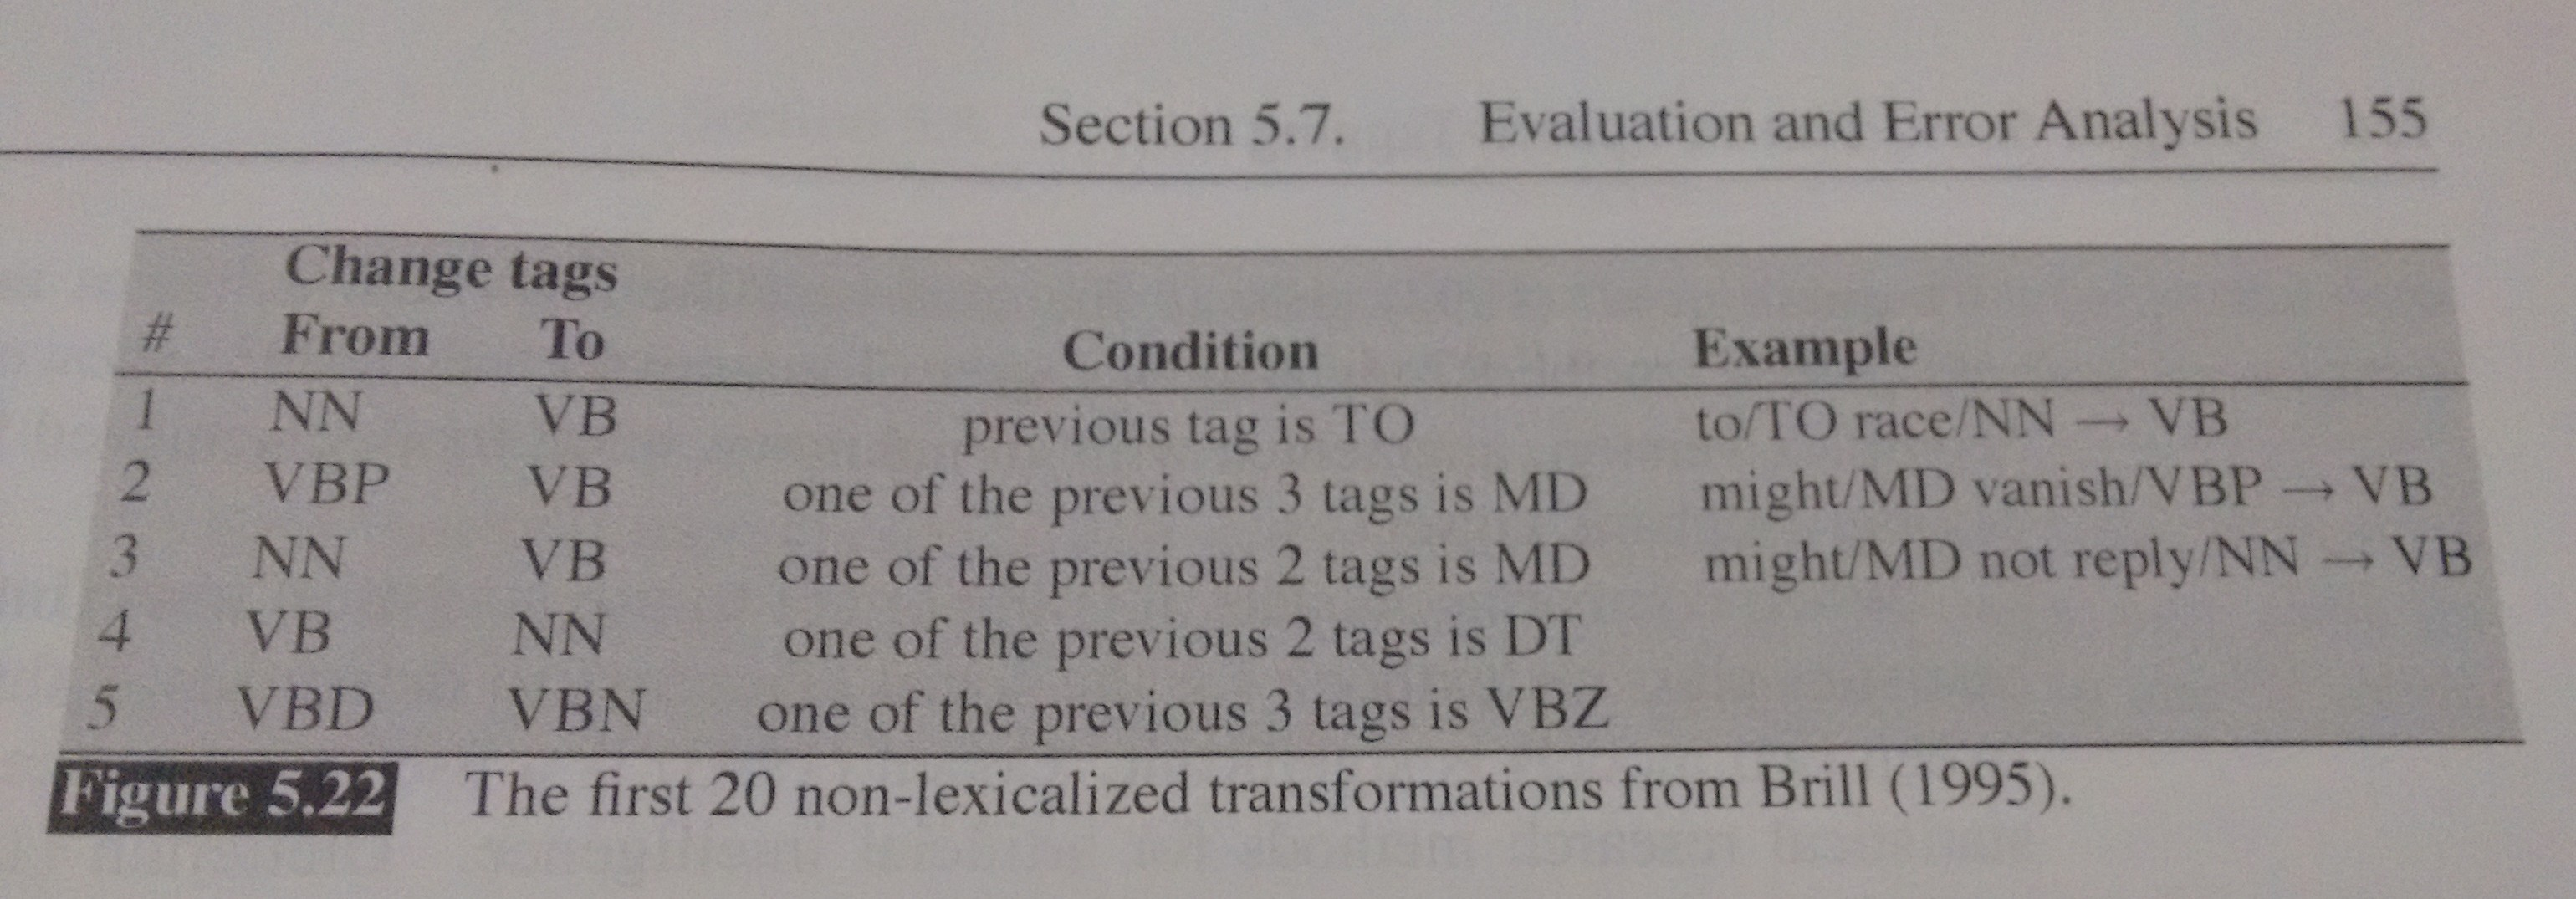
\includegraphics[width=0.9\textwidth]{Brill-3.jpg} \\ Note: In pure rule-based tagging, these rules will be created by linguists, based on their knowledge of language
\end{frame}

\begin{frame}
\frametitle{Brill's algorithm}
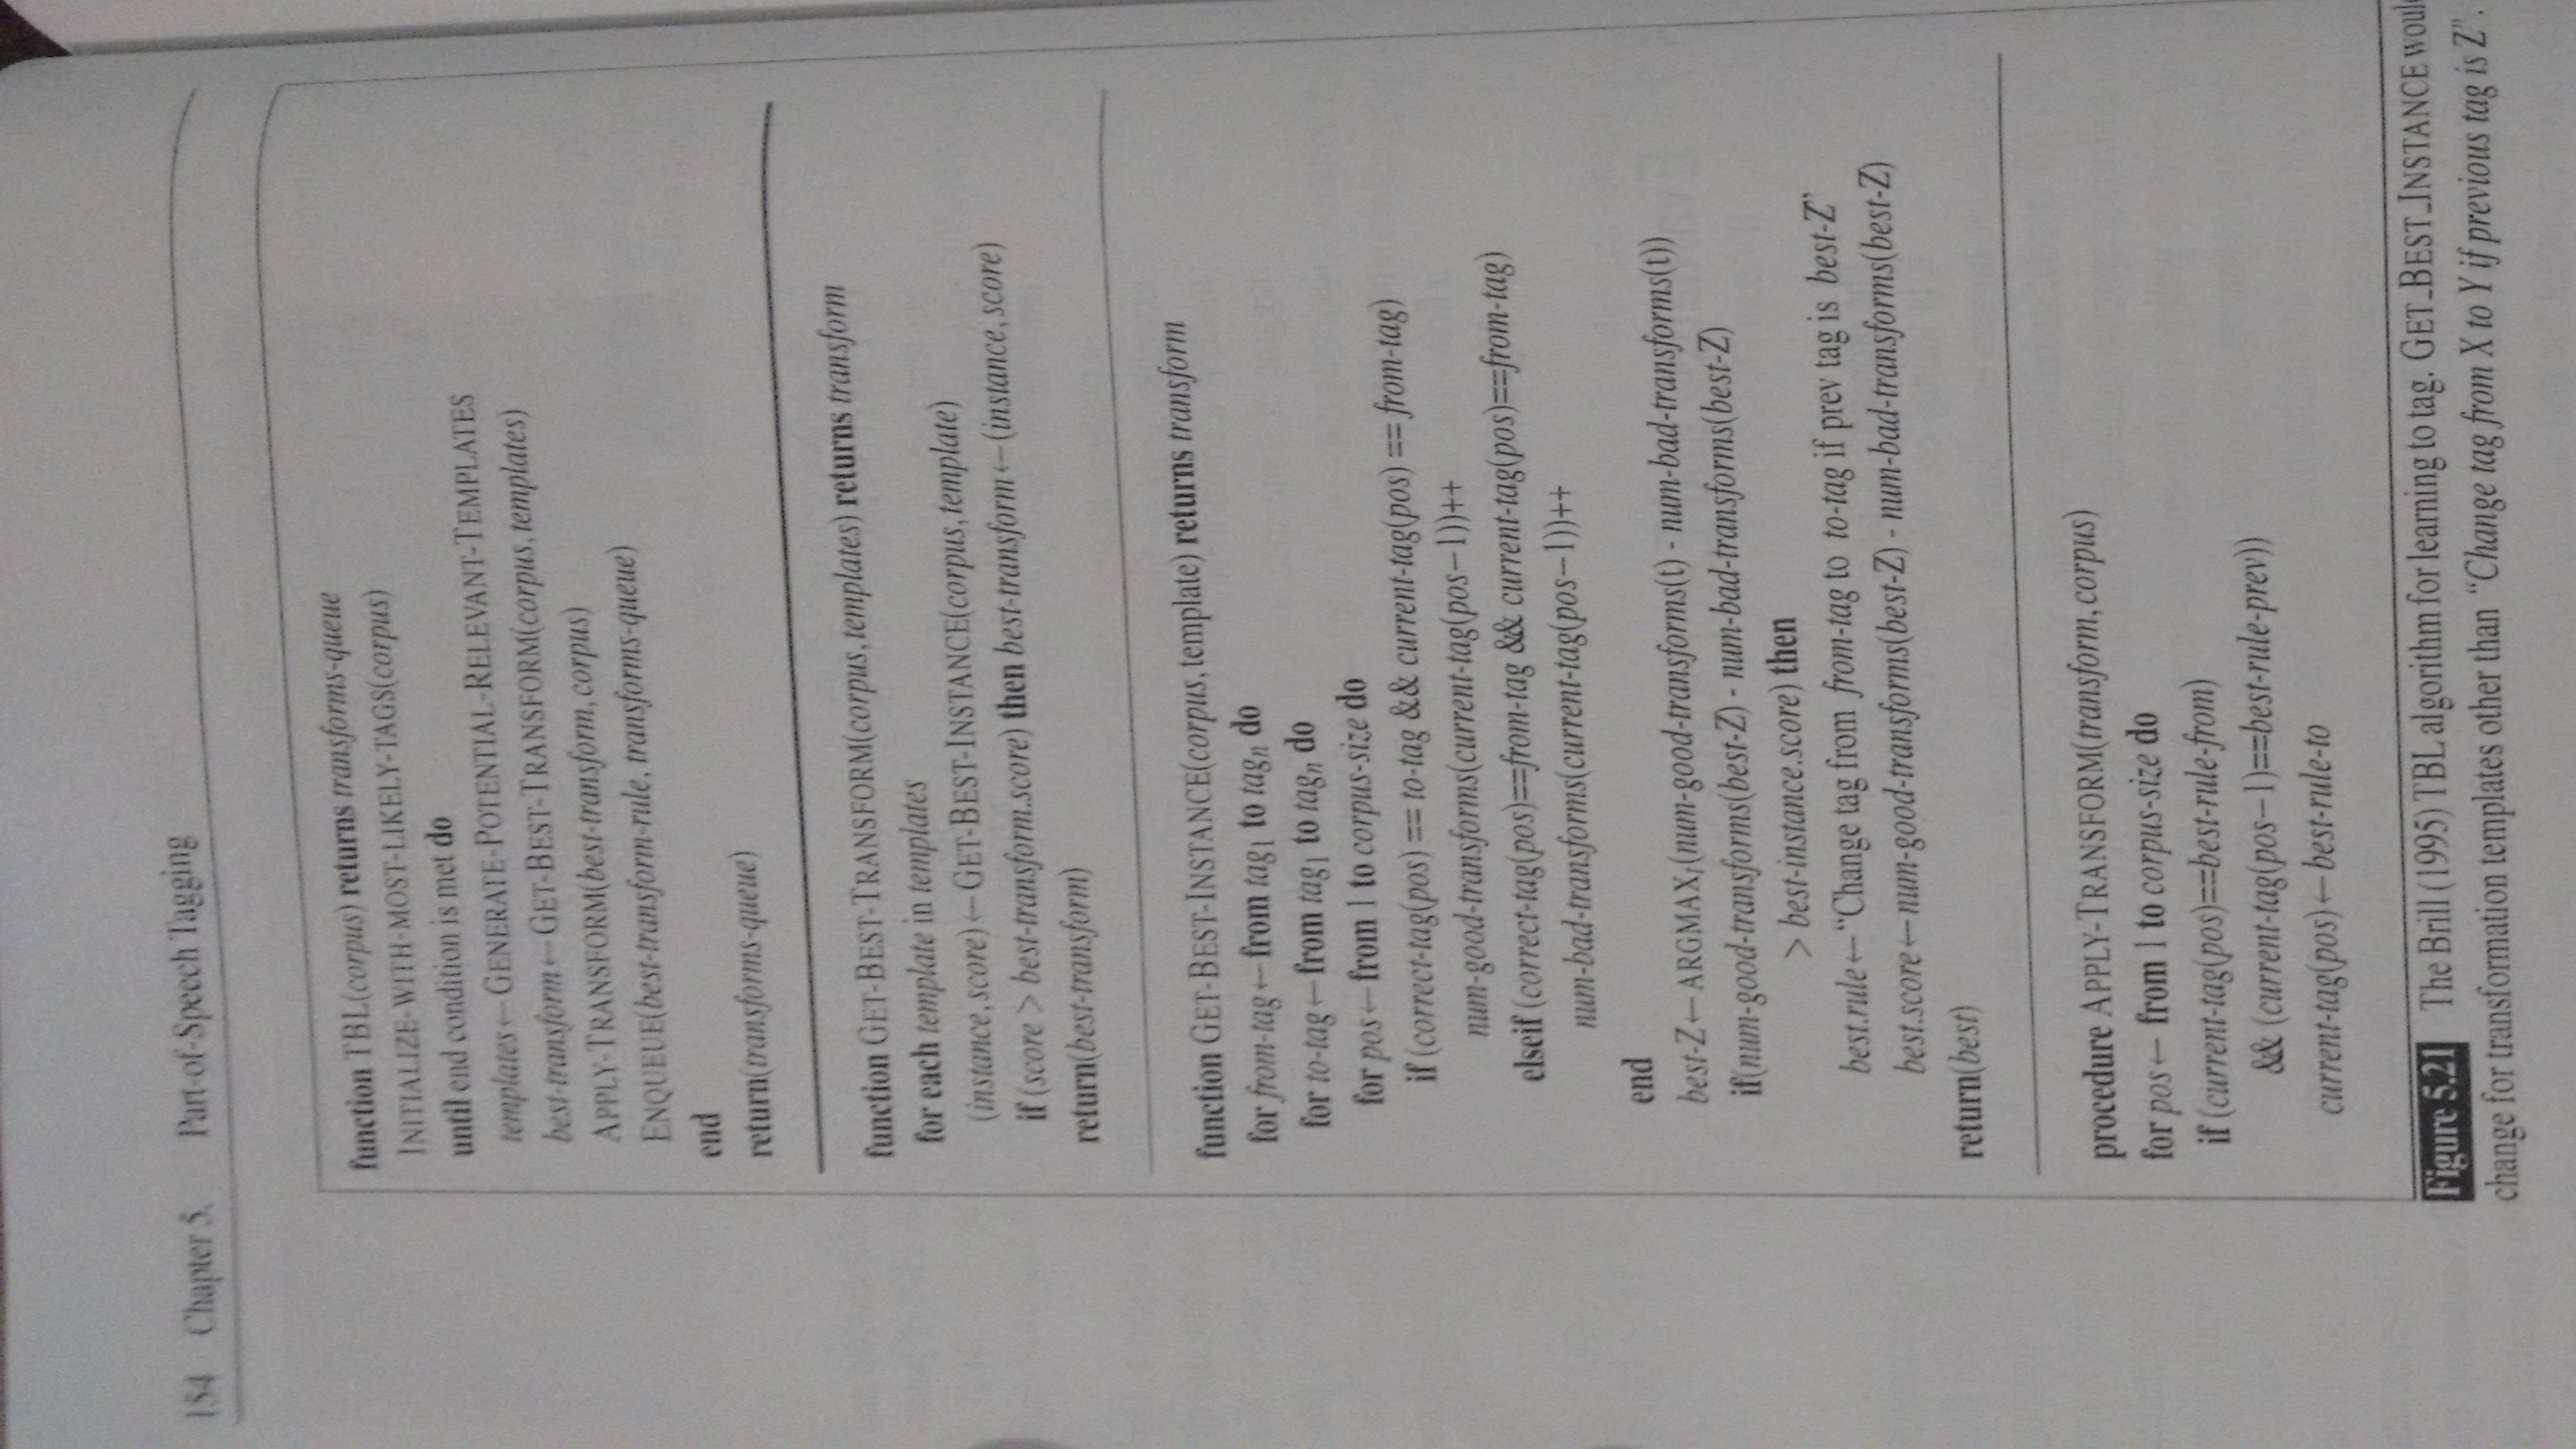
\includegraphics[width=0.75\textwidth,angle=-90,keepaspectratio]{Brill-2-b.jpg}
\end{frame}

\begin{frame}
\frametitle{To know more on TBL based tagging}
\begin{itemize}
\item Brill's 1995 paper \url{http://www.aclweb.org/anthology/J95-4004}
\item Brill Tagger implementation in NLTK: 
\begin{enumerate}
\item \url{http://www.nltk.org/_modules/nltk/tag/brill.html}
\item \url{http://www.nltk.org/_modules/nltk/tag/brill_trainer.html}
\end{enumerate}
\end{itemize}
\end{frame}

\begin{frame}
\frametitle{}
\begin{center}
\Large Evaluating POS taggers
\end{center}
\end{frame}

\begin{frame}
\frametitle{Evaluating POS taggers -1}
\framesubtitle{Intrinsic Evaluation}
\begin{itemize}
\item Tagging accuracy is the measure to evaluate the performance of a POS tagger.
\item Usually, there is a gold-standard test set which is used as a bench mark to compare all POS taggers that are developed for a given language.
\item If your tagger identifies 90\% of tags in this test set correctly, your tagger's accuracy is 90\%.
\item English POS taggers currently report up to 97-98\% accuracy with that gold standard test set.
\item Is 97-98\% good? \pause
\item What is good depends on what is the baseline and what is the ceiling.
\end{itemize}
\end{frame}

\begin{frame}
\frametitle{Evaluating POS taggers - 2}
\begin{itemize}
\item Baseline: Choose the most likely Unigram tag for a given word.
\item Ceiling: How well do humans do on this task? How much is the agreement between two humans doing manual POS tagging?
\item Note: This ceiling is under the assumption that computers cannot beat humans. But there are some tasks where computers are better than humans. 
\item So, this ceiling is not a universal ceiling for all NLP tasks.
\end{itemize}
\end{frame}

\begin{frame}
\frametitle{Evaluating POS taggers - 3}
\begin{itemize}
\item Let us say my baseline is 80\%. My POS tagger gives an accuracy fo 85\%. My ceiling is 87\%. Is the tagger doing well? \pause
\item Let us say my baseline is 75\%. My POS tagger gives an accuracy of 85\%. My ceiling is 95\%. Is the tagger doing well? \pause
\item Let us say my baseline is 80\%. My POS tagger gives an accuracy of 81\%. My ceiling is 100\%. Is the tagger doing well? \pause
\item Let us say my baseline is 30\%. My POS tagger gives an accuracy of 81\%. My ceiling is 100\%. Is the tagger doing well? 
\end{itemize}
\end{frame}

\begin{frame}
\frametitle{Evaluating POS taggers - 4}
\framesubtitle{Extrinsic Evaluation}
\begin{itemize}
\item Important thing to note: Having a good test-set accuracy does not mean the best tagger is always the best on any random sentence in English language. This is just a benchmark.
\item It is like the grades you get in school. Just one measure of evaluation. Does not cover all aspects. 
\item So, although it can be used to compare different taggers, the ultimate evaluation is the extrinsic evaluation - how it works in the real setting it is meant to be used. 
\item If you are not developing a POS tagger, you should bother about evaluating a tagger for the application you intend to use it ..
\item and not about how a tagger does on a standard test set which is not from the genre/domain etc that you want to use it in. 
\end{itemize}
\end{frame}

\begin{frame}
\frametitle{POS Tagging - Resources}
\begin{itemize}
\item Chapter 5 in Jurafsky and Martin provides a good theoretical foundation. Chapter 6 has more advanced stuff about statistical modeling.
\item Chapter 5 in NLTK Book provides a lot of practical information on using different POS taggers, and the training process.
\item Radev's Week 7 lectures in Coursera course provide a resource you can play and replay as many times you want (unlike a regular classroom lecture)
\item If you are able to finish Assignment 3, you are all set to analyse what tagger works for your purpose (if you want!), what you need if you want a customized tagger (for learner text) etc. 
\end{itemize}
\end{frame}

\begin{frame}
\frametitle{Practice Exercises}
\begin{itemize}
\item Chapter 5 in NLTK book: go through the examples. Try out the various POS taggers in NLTK, and try to do some of the problems at the end.
\item Go through problems in Problem Set 4 - See how many of them sound straight forward and start doing one of them.
\item Explore how Regular Expressions can be useful for POS tagging.
\item These slides on NLTK POS taggers is useful: \url{https://goo.gl/O3dNl3}
\end{itemize}
\end{frame}

\begin{frame}
\frametitle{Next Class}
\begin{itemize}
\item Revision of concepts so far
\item Planning for a tutorial session
\item Discussion about ideas for final projects
\end{itemize}
\end{frame}

\end{document}



